\chapter{Related Work}
\label{chap:related_work}

In this section we are going to provide and introduce the most recent projects and research that shed light on the integration of the three domains. However we are not going to only look on similar architecture but also we will see some similar use cases of real time face detection and recognition for access control. Convergence of the three domains is not by chance therefore in this section we will also list the ideas and benefits that bring the three domains together. 
The ESP EYE development board  provides the basis and the motivation to put more effort on this project. It supports image transmission via Wi-Fi and debugging through a Micro-USB port. 

\section{Synergy of the trio: IoT, AI and Blockchain }

In order to give a better understanding of IoT, AI and blockchain, it mirrors to think of them as an interconnected biological process. IoT is like our brain, which senses billions of connected devices in our planet while producing a universe of new data. AI being the rationale part of the brain. It will be thinking while analyzing data and make a decision based on that. On the other hand blockchain makes me think of memory which stores information in the growing list of blocks.
\subsection{An overview of IoT}

IoT is transforming the world of things around us into a world of sensors that speak about the things. Practically almost anything can be equipped with a sensor and make the things smart. In terms of IoT the sensors are not just used to detect and measure but they are also to respond to changes thanks to the proliferation of internet-enabled devices which are embedded with computational power. 

The number of IoT devices took over the population worldwide since 2008. Based on (ref123) the number of IoT devices is expected to increase and reach around 31 billion by the end of 2020. However this number is not expected to ever stop but it will be double by the end of 2025 as depicted in Figure~\ref{fig:num_of_iot} (ref124).

Most IoT devices run on microcontrollers or microprocessors with very minimal processing power which makes them less powered than a smartphone. The reason behind is not that such devices cannot be equipped with more processing power but to be energy efficient and run with mimimal power on battery and reducing environmental impacts of the energy use. With such growing number of IoT devices in the near future it will eventually pose a challenge even without increasing the processing power of such devices. Eventualy there will be a high demand of developing a green communication accross the network (ref126). This will at some point also affect the developers IoT devices who will have to find more lightweight programs to run high consuming energy programs such as deep learning. As a result different algorithmic approaches are taking place and more efficient algorithms are being developed (ref128).






\begin{figure}[!htb]
    \centering
    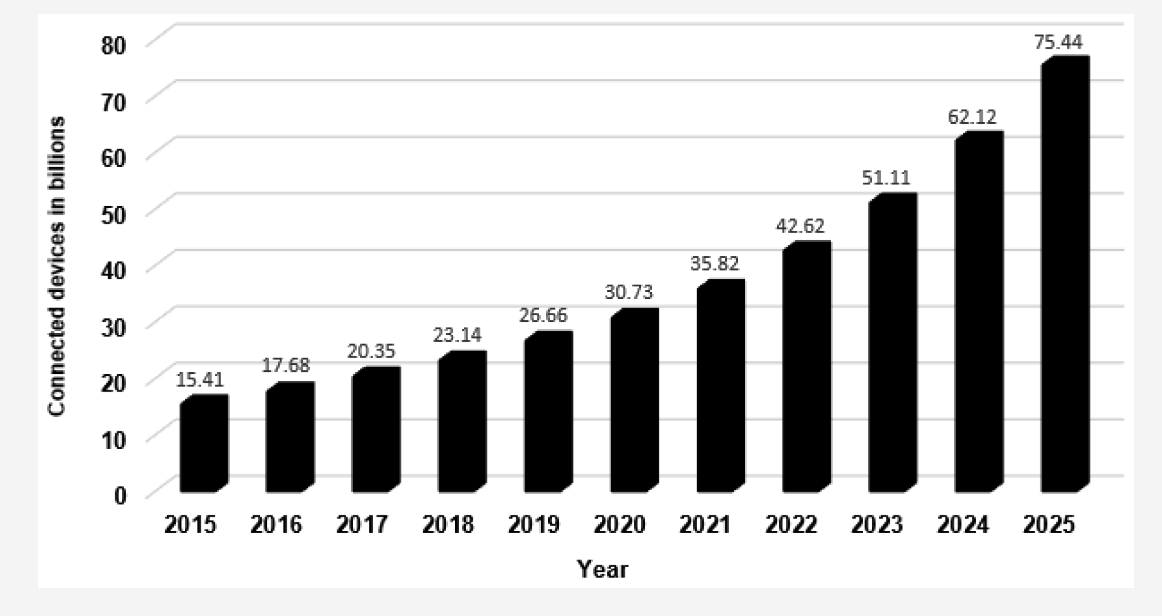
\includegraphics[width=1\textwidth]{figures/number_of_iot.png}
    \caption{The growth of IoT devices from 2015 to 2025 ref(img1)}
    \label{fig:num_of_iot}
\end{figure}


We would like to mention a number of common characteristics that most IoT devices share: 

\begin{itemize}
    \item Connectivity - with the help of a number of protocols they can communicat with each other.
    \item Heterogeneity: a variety of devices and objects including communication protocols
    \item Unique identity: a unique identifier for each device 
    \item Big data: IoT number one source of big data 
\end{itemize}

However IoT suffers from its typical architecture design which is the centralized architecture. These centralized server either on the cloud or on premise manages and deals with all requests coming from various nodes. This architecture comes with multiple challenges: scalability issues, security and privacy challenges and issues with the analysis of big data (ref130). 

\subsection{Enabling Deep Learning in IoT}
AI has become a buzzword and one of the topics that has a significant impact on many different domains. In Figure~\ref{fig:ai_terms} depicts the relationship between Artificial Intelligence, Machine Learning and Deep Learning. In simple words AI encapsulates the imitation of human intelligence by computers. Machine learning is the technique used to allow computer programs to access data and use it to automatically learn and improve from experience. The neural network involves a large number of processors operating in parallel arranged in tiers , in the same way neurons in our brain works. While deep learning employees neural networks but with many layers of neural networks. 


\begin{figure}[!htb]
    \centering
    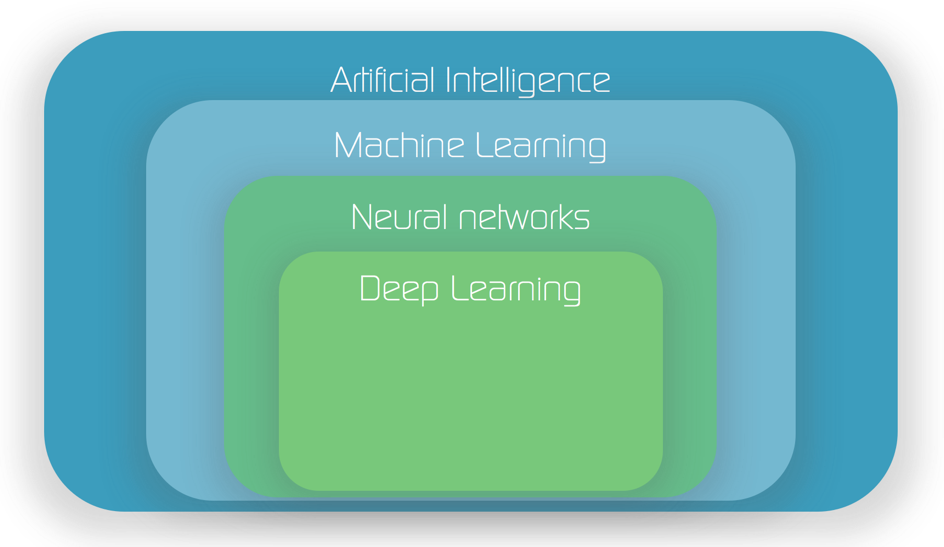
\includegraphics[width=1\textwidth]{figures/ai_classification.png}
    \caption{Relationship of AI terms.(refimg12)}
    \label{fig:ai_terms}
\end{figure}
We already know that AI can solve and make sense of the immense amount of data produced from IoT devices. However the main question for research appears “How to deploy neural networks directly on these tiny devices? Therefore there is an opportunity and challenge at the same time to run machine learning on such tiny IoT devices based on microcontrollers. By running machine learning on these tiny devices, we can directly perform real time data analytics in the device itself, therefore avoiding the need to store all the data generated from the IoT device. Typically commercial use cases of smart IoT devices often offload the Artificial Intelligence part to the cloud. 
One of the most recent study(ref321) that worked on this direction tested two approaches with deep learning: 
\begin{itemize}
    \item Offloading deep learning platforms to the cloud
    \item Migrate deep learning to an IoT device
\end{itemize}

The two approaches were tested and look from two different perspectives,  whether offloading machine learning can reduce energy efficiency and satisfy the real time requirements of object recognition. 
In the first approach they used convolutional neural networks on the cloud, while the Jetson TX1 was responsible to just take images and forward them to the cloud. The results show that executing machine learning in the Jetson TX1 consumed more energy compared to the offloading to the cloud. However offloading AI to the cloud also comes with drawbacks, it has lead to a range of latency starting from 2 seconds that goes up to 5 seconds which is far higher compare to the execution of AI in the Jetson TX1 itself. This leads to conclude that the variability of response time make it quite unreliable and not useful for real time AI processing. 

Furthermore MIT researchers ref(mit123) have implemented a sytem called MCUNet, which has a high potential to bring deep learning in much smaller devices like tiny computer chips despite their limited memory and computational power. 

\subsection{Intersection of Blockchain and AI}

There is a high research on Blockchain and AI but analysed in isolation and in various domains and applications. Some research ref(17) focus on the application of AI in the Blockchain for making blockchain more efficient for instance, consensus mechanisms and better governance. However there seem to be more research and applications of Blockchain in AI. Similar to IoT, AI domain also suffers from security, its centralized architecture and resource limitations. This is exactly what blockchain is looking to solve. There is a lot of discussion and research in this area, however most of them are reviews and solutions that do not provide a use case or implement such solutions. In order to have a global image the Table ref() describes the features of the two technologies and the benefits of integrating such features.

There is another interesting contribution (ref) that came up with an AI blockchain platform to fight the propagation of fake news. This platform allows publishers to setup a distribution platform in the blockchain while AI will be monitoring on the actors who are adding news to the blockchain. Expectation is that the blockchain will server as the "factual database" to trace back the news. So the news which cannot be traced back to the blockchain will be automatically considered fake. 




\begin{table}[hbt!]

    
    \begin{tabular}{  p{4.4cm}  p{4.4cm}  p{5.4cm} }
      
\textbf{Blockchain}      
& \textbf{AI}   
& \textbf{Benefits of blockchain} \\\midrule
Decentralized & Centralized        
& Enhanced Data Security \\\hline

Immutable & Probabilistic       
& Collective Decision making \\\hline


Data Integrity & Volatile      
& Decentralized Intelligence \\\hline

Resilient to attacks & Data, knowledge and decision centric     
& High Efficiency \\\hline

Deterministic  &
Changing      
& Improved trust on robotics decision \\
        \bottomrule
    \end{tabular}
    \caption{Benefits of integrating blockchain into AI  (adopted from \ldots%\citealt{crouch2012doing}
    )}
    \label{crouch}
\end{table}

\subsection{Integration of Blockchain with IoT}

We have already listed a number of issues that IoT world is facing, which mainly is the centraized architecture, security and privacy. Therefore pretty much of the research is focused in this area, typically with the advantages of blockchain those gaps can be closed. For instance ref(IS) attempted to discover the security gaps that could be mitigated with the help of the blockchain to ensure the reliability and availability of the data.

Other studies (refIS) attempted to integrate crypto based blockchains such as Ethereum in their approaches. We argue here that most of the crypto based blockchains are not efficient in storing data coming from IoT devices. First users have to pay fees for each transactions and the there is a limitation in the number of transactions it can process. Although we can escape from the centralization still there is the risk of bottleneck. Therefore in our study we will be using Hyperledger Fabric a non crypto based blockchain aimed for storing data. 


































\begin{comment}

\begin{table}[!h]
\definecolor{LightCyan}{rgb}{0.88,1,1}
\definecolor{Gray}{gray}{0.9}
\newcolumntype{g}{>{\columncolor{LightCyan}}c}
\noindent\begin{tabularx}{\textwidth}{|g|l|X|}

\hline apple  & StackOverflow & Dardh \\
\hline 
\begin{itemize}
\item[--] Decentralized

\item[--] Deterministic
\item[--] Immutable
\item[--] Data Integrity

\end{itemize}

& StackOverflow &
 lots of long text. lots of long text. lots of long text. lots of long text. lots of long text. \\
\hline 

\end{tabularx}
\caption{Truth Tables and Accuracy Measures for each modeling library.}
    \label{tab:truthTables}

 \end{table}



\end{comment}

 
 
 
 \section{Use cases on AI, IoT and Blockchain}
 
 We have already described the intersections on how Blockchain, AI and IoT accommodate each other in pair, however there is a very high potential for the usage of all the three domains in one use case. With such a high number of IoT devices there is a potential to take the advantage of AI and Blockchain at the same time. Based on reforacle, every institution  which will take the advantage of exploiting these technologies, it will have the chance to radically enhance their existing processes and create entirely new business models. 
 
An interesting work ref(smartcity)  presents how the collaboration of the three domains can build a sustainable smart city. Given the many issues people in urban areas face, the concept of the sustainable smart city brings new opportunities for the application. With their new approach they aim to have a transparent monitoring system for measuring pollution which in turn will help raise awareness to the population. 

In another use case the authors (refhomeauto) propose an IoT based home automation and surveillance system. In this setup they have employed a raspberry pi, a camera attached to it and a DC motor for controlling the door. The video surveillance is not detecting or recognizing people, so the burden falls into the owner who through the help of a front end will be able to open the door. Therefore compare to our solution there is no AI and blockchain integrated. 


A use case that pretty much is matching with our use case is a design and implementation of a camera based sensor for room capacity monitoring. The aim of it is to count the number of people present in a room with the help of a raspberry pi and a camera. In Figure~\ref{fig:raum} we can see the architectural overview. 

\begin{figure}[!htb]
    \centering
    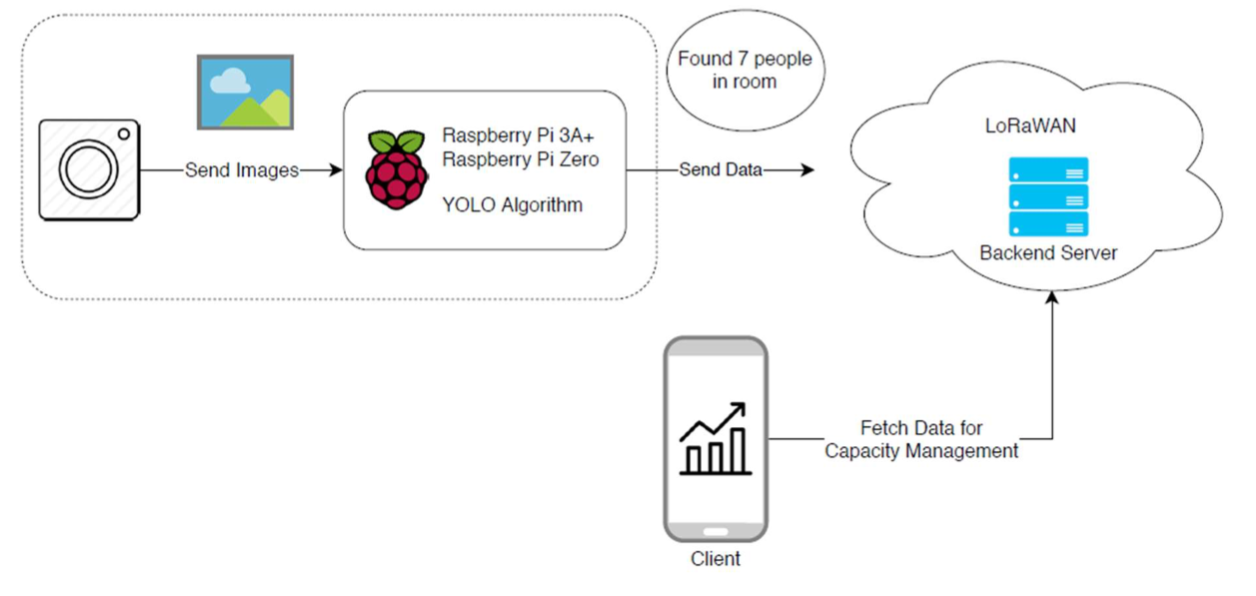
\includegraphics[width=1\textwidth]{figures/raumbelegung.png}
    \caption{Architectural Overview(ref)}
    \label{fig:raum}
\end{figure}

Their architecture employees AI and IoT. This use case was designed and implemented by a group of students at FHNWS who employed a raspberry pi equipped with camera and lora gateway. The role of camera is to just take pictures and after that some machine learning algorithm will analyze the image and find the number of people in the room. Once done the data is then send to a LoraWan Server. To achieve that they have attached a LoraWan antenna to the RPI and eventually with a front end they can monitor the room. So face detection happens in the RPI, the algorithm counts the number of people in the image and sends it to the Lorawan Backend Server. From here we can conclude that the issue of centralisation is still open, data is being stored in a database, security issues are not tackled enough. Besides there is also the need for a RPI to be placed in a room as the camera is attached to it and that needs power to run. 

With out proposed architecture we are not only going automate the IoT-based surveillance system but provide a robust solution that will take care of the leaks that AI and blockchain will be able to neutralize. 


\chapter{Face Detection and Recognition in IoT devices}
\label{chap:face_detection}
\section{Background of real time face recognition in low powered IoT devices}
Monitoring and tracking people and their activities with the current approaches of the surveillance system normally generate enormous amount of data coming from Internet of Things devices. This leads to a number of issues that need to be treated well, data migration from camera over a limited bandwidth for face detection and recognition leads to high latency  and the camera positions need to be placed near the electrical plug as they require a lot of power. Therefore this approach leads to generating a lot of data while transferring it to a different source for face detection and recognition. Besides many public places use surveillance camera for video capture based on motion detection, which means that once someone approaches near the camera it will start recording and throughout the day you can imagine how much volume of data can be generated. 
In this chapter we will guide you through the existing algorithms for face detection and recognition and then we will see the algorithms that are implemented for the resource constraint devices or IoT. Therefore we will also discuss the reason behind choosing to deploy the face detection and recognition algorithm in the ESP EYE itself. In addition the Multi-task Cascaded Convolutional Networks (MTCNN) and  Human Face Recognition Model (FRMN) for face detection and recognition will be described in detail. 


\subsection{The generic framework for face detection and recognition}


Face detection is normally the first step towards face recognition or verification as it can be seen in  Figure~\ref{fig:framework}. Basically the framework follows a two step process: face image detecting and face recognizer. In the first process an image is taken from the camera which searches for human faces in that image then the algorithm localizes the face from the background image. This process happens continuously which means if there is no face detected the takes the next image and does the same. The image when no face is detected is deleted from memory. The next process assumes the image is taken and a face has been detected then the face recognition will start. In this phase another algorithm will take place in order to determine who are the persons in that image. During both processes, algorithms extract features or a pattern which is the key step of the algorithm. Feature extraction is the process is essential for localizing facial components such as mouth, nose, eye and others. 

\begin{figure}[!htb]
    \centering
    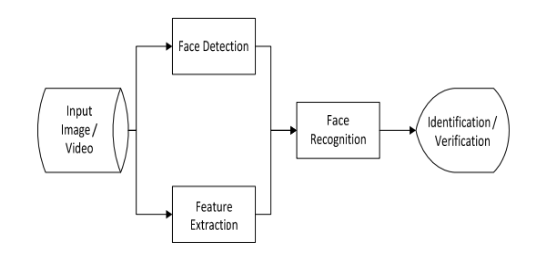
\includegraphics[width=1\textwidth]{figures/framework.jpg}
    \caption{ Face detection and recognition.}
    \label{fig:framework}
\end{figure}


\subsection{Existing  algorithms  for  face detection and recognition}

There are a number of algorithms that have been developed and now used to tackle the face detection and recognition issues. We would like to mention a number of successful algorithms which are widely used and they are: 

\begin{itemize}
    \item \textbf{Principle Component Analysis (PCA).} It is a statistical approach and one of the simplest in face recognition systems. In this approach images with detected faces are transformed into eigenfaces. Eigenface is a method that determines the variance of faces from a collection of images. The main idea behind is to linearly project images onto a lower dimensional images. 
    
    
    \item \textbf{Linear Discriminant Analysis (LDA).}
   It is a method used in pattern recognition and machine learning by finding a linear combination of features. It used for dimensionality reduction and performs very well in face recognition. It finds a projection transformation by maximizing the between-class distance and minimizing the within-class distance. 
   
   
   
    \item \textbf{Skin colour based algorithm.}
    As the name says, it uses skin color as a feature for face detection and it is fast, self adaptive algorithm. From the input image it uses color space for the skin region. A bounding box is drawn to extract the face from the image.
    
    
    \item \textbf{Wavelet based algorithm}
    In this method the image is cut up into a subset of frequency components and to each component is applied a mathematical function. One of the widely known algorithm is the Gabor wavelet.
    \item \textbf{Artificial  neural  networks  based  algorithm}
    Typically face recognition is achieved with the help of deep learning more specifically the Convolutional Neural Network. Through a multy-layered network which performs a specific task using classification.
\end{itemize}


\subsection{Hardware requirements for running real time face recognition}

It is important to mention that a typical computer or a laptop possess an AMD processor, while a raspberry pi and smart phones and some other devices like watches are equipped with a ARM processor. Obviously ARM architecture offers lower performance compare to AMD, but there is a reason behind, the ARM processors consume less power than AMD processors. Performing real time recognition on both AMD and ARM is not an issue, both can handle them. However both processors need power either plugged or if on battery they can last max one day long. In contrast the low powered IoT devices can run for years with a typical voltage of 3.6 V. Therefore to our knowledge so far it is not possible to perform real time recognition with a processor other then the above mentioned, AMD and ARM. 

ESP EYE is the first device to perform real time face recognition. However, this does not mean that the face detection and recognition algorithm have been used one to one. ESP EYE is one of its kind that comes with ESP WHO platform which supports both face detection and face recognition. The ESP EYE is equipped with Tensilica LX6 dual core processor. To our knowledge this is the only device that can perform real time face recognition in a microprocessor that lies out of the two classes AMD and ARM processors. 

\section{Face detection with deep learning using Multi-Technology Network Management (MTNN)}

MTMN refers to both MTCNN (Multi-task Cascaded Convolutional Networks) and MobileNets. There are a number of deep learning methods that have been implemented and paved the way for face detection but MTCNN is a framework which integrates both face detection and alignment. With the help of MobileNets it builds light weight deep neural networks which uses depth-wise separable convolutions for face detection.


\subsection{MTCNN a three layer CNN model}

MTCNN is one of the state of the art approaches which is described and published in the paper "Joint Face Detection and Alignment Using Multitask Cascaded Convolutional Networks" ref(mtcnn) in 2016. MTCNN is popular because it has achieved 95 percent accuracy on a range of banchmark datasets. MTCNN is a novel approach because it performs a lightweight Convolutional Neural Network based framework which actually performs simultaneously face detection and alignment whereas in other CNN-based frameworks face detection and alignment are two distinct processes.   
Due to its lightweight CNN architecture it can perform in real time which is possible to run it in an ESP32 chip. 

The process consists of three stages of Convolutional Neural Networks that are able to detect faces and landmark location such as eyes, nose, and mouth : 

\begin{itemize}
    \item \textbf{P-net} 
    \item \textbf{R-net} 
    \item \textbf{O-net} 
\end{itemize}


The Figure~\ref{fig:mtcnn} adapted from the paper depicts a summary of the three layers with the output of each layers on the right side. The three mentioned models perform independent of each other, the output of each is used as an input of another. 
First of all once the image is captured it will be scaled into multiple different sizes based on different scaling ratios which forms a collection of images called Image Pyramid similarly as in Figure~\ref{fig:pyramid}. This will allow the model to learn different image scales effectively. This type of image processing is used extensively because it makes it easier to detect faces no matter how far or close they stand in the image.


\begin{figure}[!htb]
    \centering
    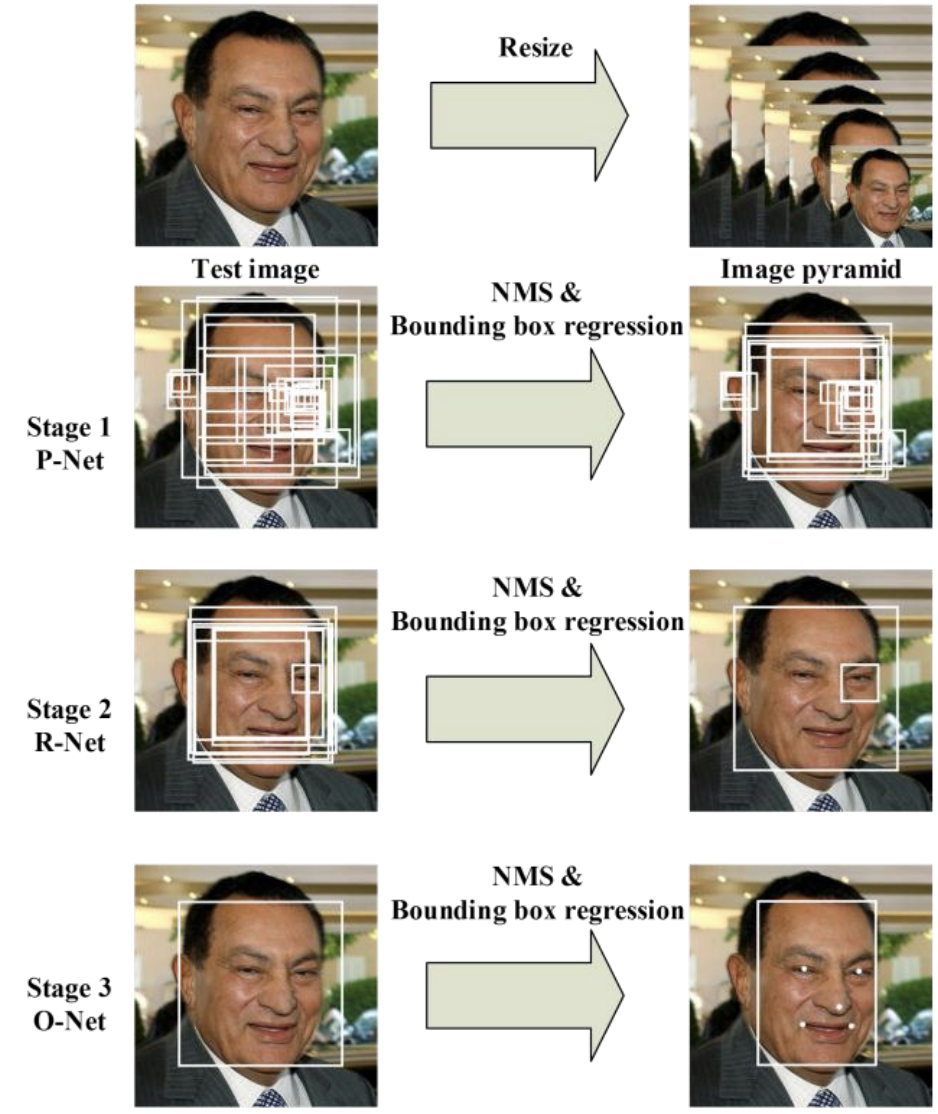
\includegraphics[width=1\textwidth]{figures/mtcnn.png}
    \caption{ Pipeline of MTCNN that includes three-stage multi-task deep convolutional networks.}
    \label{fig:mtcnn}
\end{figure}

\begin{figure}[!htb]
    \centering
    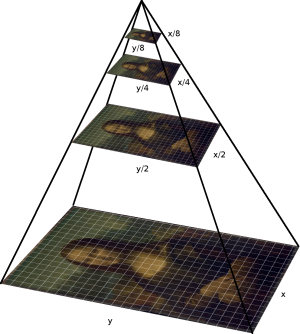
\includegraphics[width=1\textwidth]{figures/pyramid.png}
    \caption{ Image rescaled in a form of a pyramid}
    \label{fig:pyramid}
\end{figure}

\subsubsection{Proposal Network or P-net}

The first stage of Proposal network (P-Net) as depicted in Figure~\ref{fig:3stages} is a full convolutional neural network which extracts face candidate regions from images at various scales and bounding box regression vectors. Bounding-box regression is a technique for refining or localizing boxes in objects. In other words it is a rectangle which is drawn over the image to emphasize the face. For each of the scaled image that reside in the image pyramid it runs a 12x12 kernel which starts in the top left corner or at these coordinates (0,0) to (12,12). This portion of the image 12x12x3 will be the input for P-Net as it can be seen in Figure~\ref{fig:3stages}. To this image then is run another kernel of size 3x3 and then it produces feature map or smaller images depending on the stride. For example in the first filtering it produces feature maps of size 5x5. The stride is the number of jumps or pixels that the kernel moves to apply a filter. In the order to deliver a 5x5x10 from 12x12x3 with a kernel 3x3 the stride is 2. Therefore stride plays a role in time complexity of the algorithm, the smaller the stride the higher the time complexity. From this 12x12 portion of a scaled image from pyramid the P-net will output the coordinated of a bounding box of there is a face. Before releasing the last output bounding box coordinates a number of similar boxes are filtered out with lower confidence and only the ones with higher confidence are kept. The bounding boxes left may still overlap as in Figure~\ref{fig:non-max}, therefore we need the one that perfectly covers the face. To do that the non-max suppression technique is applied which reduces the number of boxes by taking the best fit and not the one the network is more confident in. 




The aim of the this network is to check whether there is a face in the input and output the face frame or box with the four coordinates. In the face classification the network outputs the probability of being a face and not being a face and both values add up to 1. The bounding box holds the exact position of the box with coordinates. 


\begin{figure}[!htb]
    \centering
    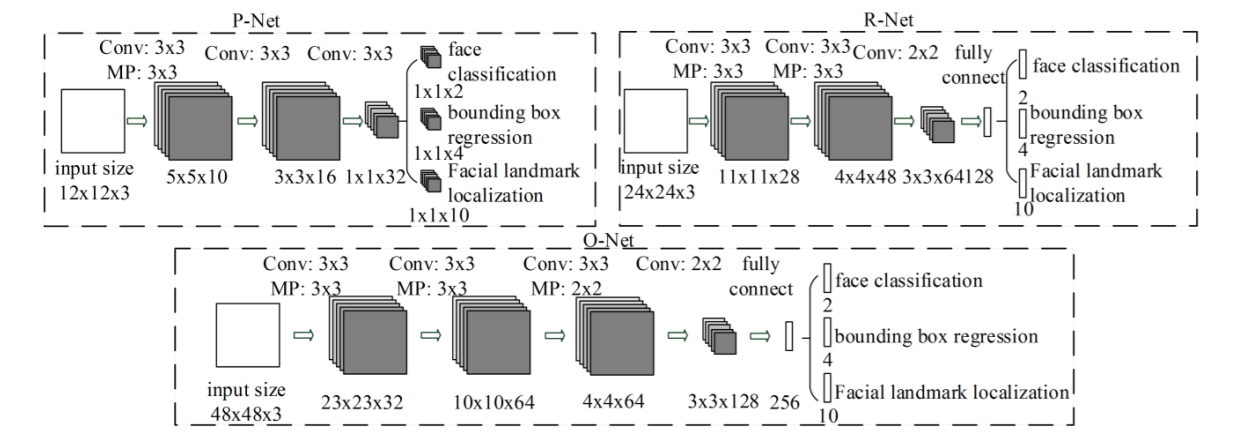
\includegraphics[width=1\textwidth]{figures/3stages.png}
    \caption{ MTCCN: P-Net, R-Net and O-Net structure}
    \label{fig:3stages}
\end{figure}


\begin{figure}[!htb]
    \centering
    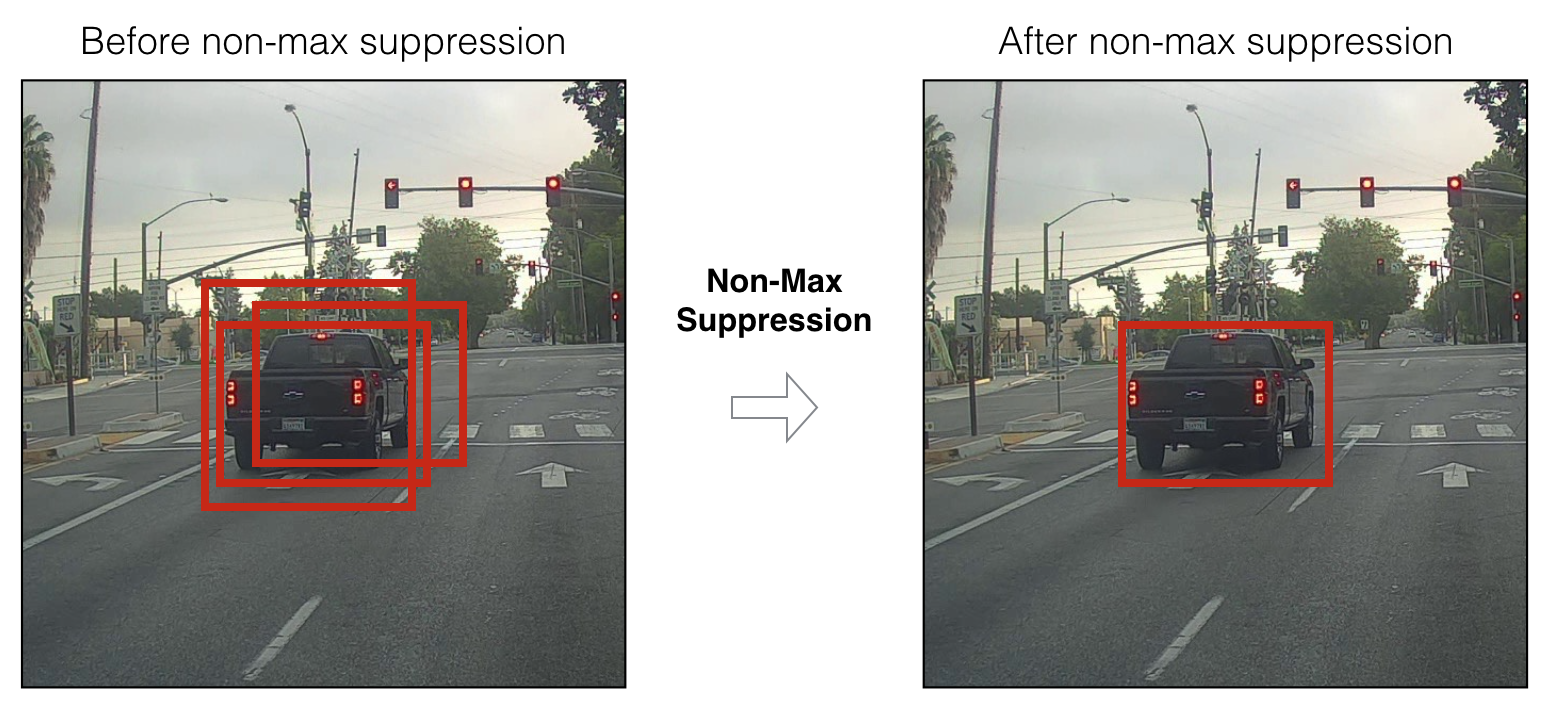
\includegraphics[width=1\textwidth]{figures/non-max.png}
    \caption{ Non-Maximum Suppression}
    \label{fig:non-max}
\end{figure}
\subsubsection{Refine Network or R-net}

The structure of R-net can be seen in the Figure~\ref{fig:3stages} which looks pretty much the same as R-net. R-net is a rough prediction of faces therefore there are a number of false positives so the aim of R-net is refinement of the bounding boxes and reduce the number of false positives.
The input of this stage is the bounding box generated by P-net which can be of different sizes. From the Figure~\ref{fig:3stages} we can see that the input size is of size 24x24x3. So regardless of the size of the bounding box it still needs to be scaled to the expected input size before sending to R-Net. Therefore the bounding boxes will be scaled to 24 x 24 pixels and now we can feed them to R-Net. Once again the same as in P-net happens, get rid of boxes with low confidence and apply the NMS on every survived box. The output is the same as of that of P-net which also consists of the tree parts: probability of being a face or not, square frames and the position of the landmarks. This stage can help to recover the weaknesses of P-net and improve accuracy by reducing the number of false positives. 


\subsubsection{Output Network or O-Net}

In the Output Network almost the same happens as in R-Net with some changes in middle layer where additional channels are added which means accuracy is also increasing. The input, feature maps are getting higher and higher in terms of pixels. The accuracy rate is expected to be higher which is proportional to the increased time complexity. In this case the output of R-Net will be the input but scaled to 48x48x3. 
Now we can already see the reason behind using three neural networks and not one. Since the final decision is received from O-Net we can directly use it and avoid the previous two networks. But the speed will be very slow since O-Net will have to do a lot of operation on all candidate windows which can be very high. With the help of P-net and R-Net a lot of non relevant windows will be filtered out from the start. From P-Net to R-Net a lot filtering happens, so the advantage here is to perform fine grained face detection only on highly probable candidate windows. To make the story short here is a summary of the whole face detection process: 
 
 P-Net:
\begin{enumerate}
  \vspace{-0.7cm} \item Image is captured by ESP EYE.
  \vspace{-0.3cm}\item Create image pyramid with multiple scaled copies of the image.
  \vspace{-0.3cm} \item Pass each image of pyramid to P-net.
  \vspace{-0.3cm} \item Candidate windows as output.
  \vspace{-0.3cm} \item Filter out bounding boxes with low confidence.
  \vspace{-0.3cm} \item Adjust the current 12 x 12 kernel coordinates to “un-scaled image” from pyramid.
  \vspace{-0.3cm} \item Non-Maximum Suppression for all kernels.
   \vspace{-0.3cm} \item Adjust the bounding box coordinates to “un-scaled image”.
   \vspace{-0.3cm} \item Candidate windows as output.
\end{enumerate}

 R-Net:
\begin{enumerate}
  \vspace{-0.7cm} \item Pass the bounding boxes
   \vspace{-0.3cm} \item Pass each image of pyramid to P-net.
  \vspace{-0.3cm} \item Candidate windows as output.
  \vspace{-0.3cm} \item Repeat step 5 to 9 of P-net.
\end{enumerate}


 O-Net: Repeat the same steps as in R-Net

\subsection{MobileNetsv2 for lightweight CNN}

MobileNet is a CNN architecture developed by researchers at Google which typically is used for in Image Classification and Mobile vision. The model is proven to build light-weight deep neural networks which uses less computational power to run. This architecture allows to run face detection and recognition for IoT devices, Mobile devices and computers with low computational efficiency without compromising the accuracy of the results. MobilNet version 2 is the recent version which comes with a research paper published in late 2018. It is a refinement of the MobileNet version 1 which make it even more powerful. 

In order to understand why this model is being used and at which step in face detection is used we would like to first give a quick recall on how convolutional neural network works. CNN is composed of neural networks as in Figure~\ref{fig:3stages} which in our case receives an image  and transform it through a series of hidden layers. Each hidden layer is made up of a number of neurons which are nothing else but mathematical functions and in terminology it is called activation function which calculates the weighted sum of multiple pixels and decides whether or not to send a signal to the next neuron. The activation function takes the weighted sum of all inputs plus the bias.

Before reaching the next neuron, a convolution or a filter is applied to the input image and a feature map is created from it. We can see in P-net in the first layer there are 10 feature maps created with a size of 5x5. That means a convolutional filter is applied 10 times to the input image, the size of the kernel in our case is 3x3. But this does not mean that the same filter is applied but different ones as in Figure~\ref{fig:filter}. This kernel slides accross all the pixels of the input image by covering all of them and at each step it computes the weighted sum and puts in the feature map or a in the newly generated image as in Figure~\ref{fig:conv}. Depending on the size of the kernel and input image the new image normally the new feature map will have a smaller size. Here is where pooling comes into play, with pooling we can upsample or downsample or change the spatial dimensions but in fact only max-pooling is performed because there we need to find outliers which is the moment the network can detect features. So the deeper we go in the image the better to detect features. When the output of the P-net was generated which is an image or candidate window it had to be upsampled because R-Net only receives image of dimensions 24x24x3. This means we are somehow zooming in the image more and more until the last network is performed. Besides we can also see that the number of filters is increasing and in the last layer of O-Net we can see feature map of dimensions 3x3x128 which means 128 filters have been applied. 
\begin{figure}[!htb]
    \centering
    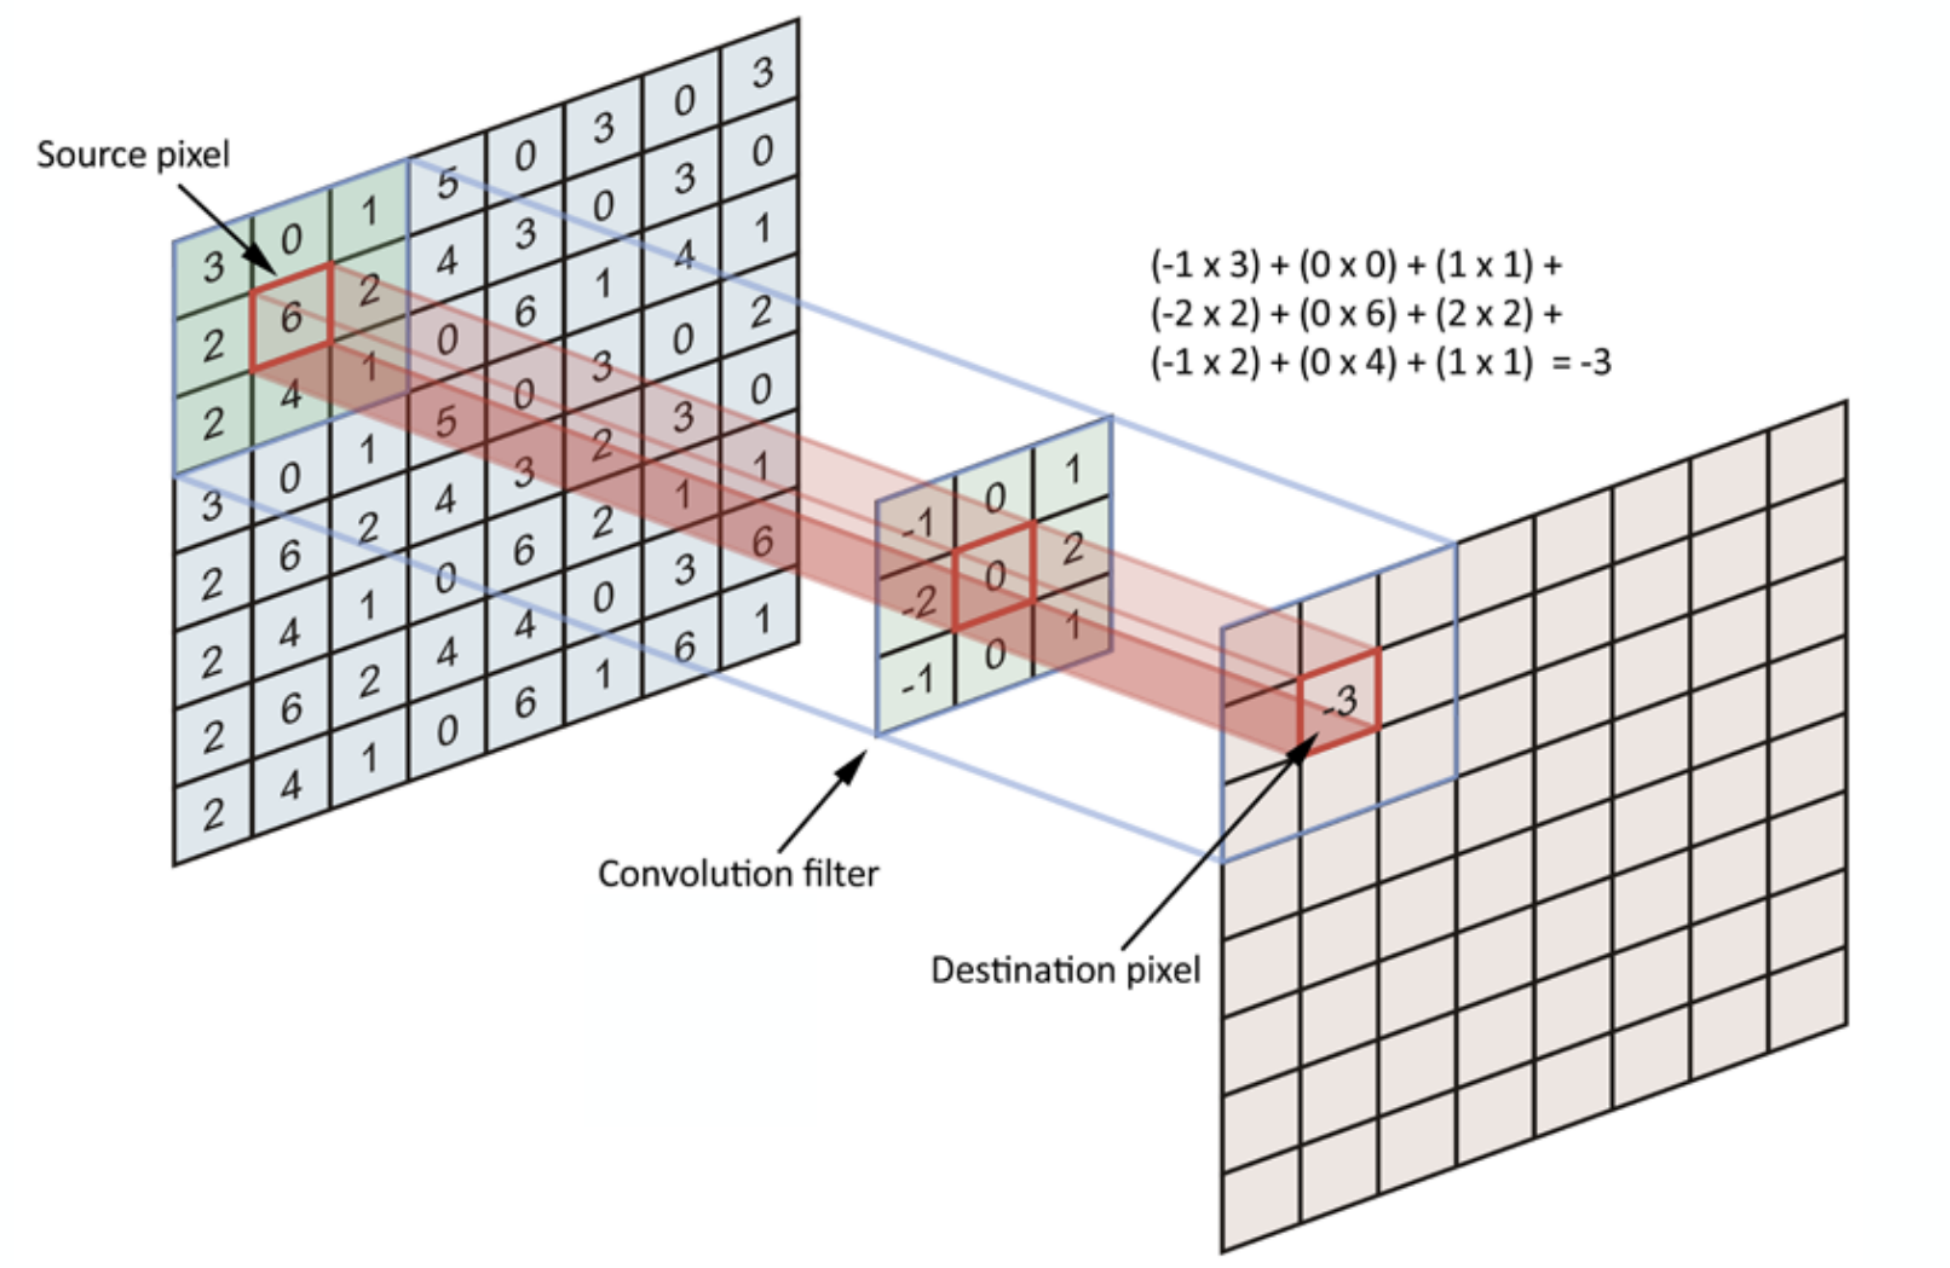
\includegraphics[width=1\textwidth]{figures/convolution.png}
    \caption{The convolution operation}
    \label{fig:conv}
\end{figure}


\begin{figure}[!htb]
    \centering
    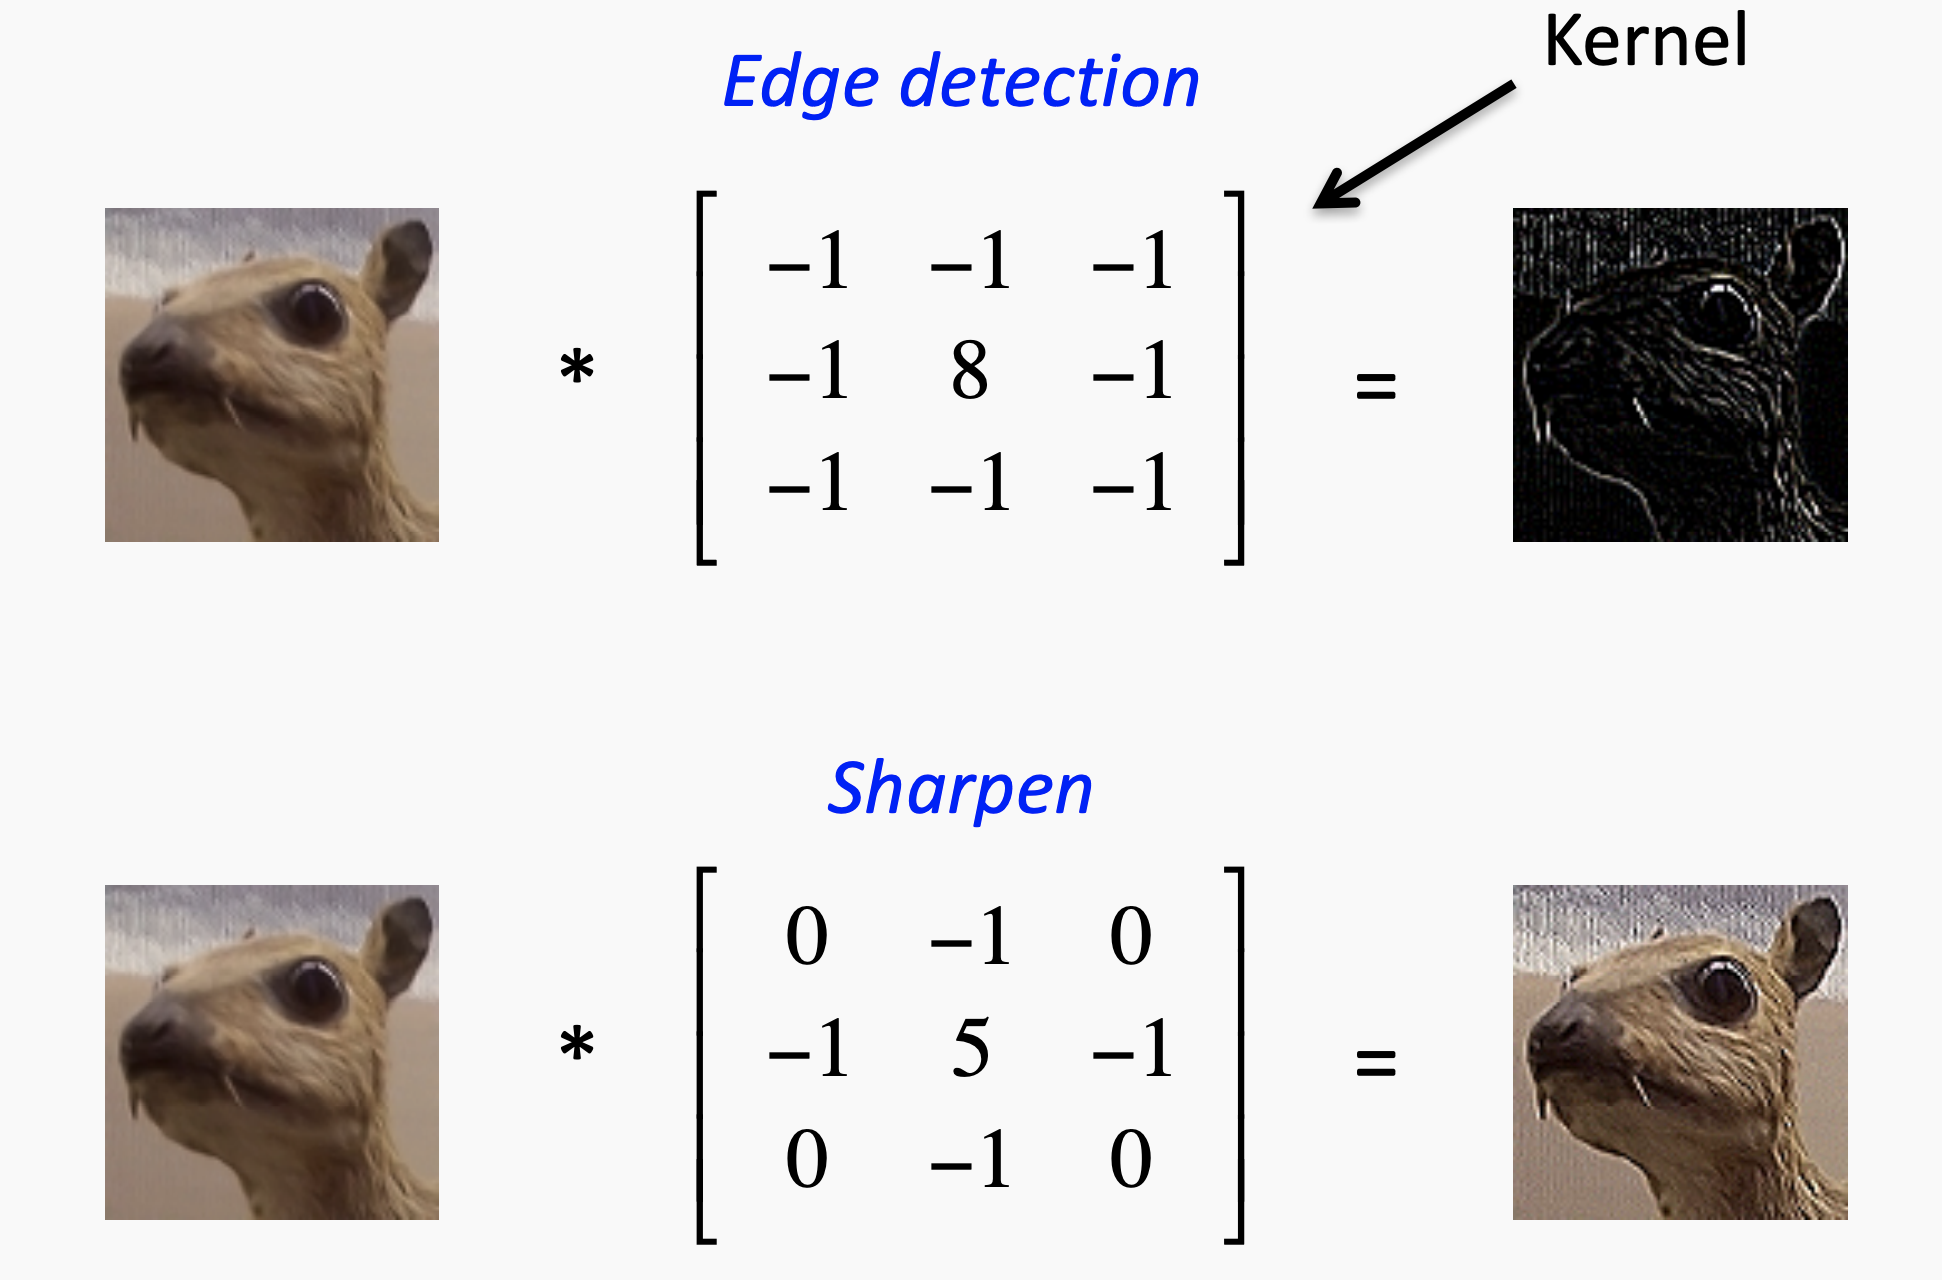
\includegraphics[width=1\textwidth]{figures/filters.png}
    \caption{Examples of filters}
    \label{fig:filter}
\end{figure}
From here we can understand the reason behind the staging. Performing the convolution to the image directly from the last stage we would need a lot of computation because filtering obviously takes time. Imagine having an image where the person to be detected is standing far away and in the image that person may cover for example only 5x5 pixels out of an image of 360x240. So applying a high number of filters in each extracted image with 5x5 pixels is not efficient. So the idea is to first apply filtering in larger parts of the image so that we can get rid of candidate windows which do not include faces.

The staging approach is quite efficient in face detection while MobileNets is essential in the way convolution is performed in applying the filters and creating feature maps. 



\subsubsection{Normal Convolution}

The main idea behind MobileNetv2 is to get high accuracy with less computational power. In the regular convolution, the convolution kernel or the filter is applied on all the channels of the input image. The input image will normally have 3 channels and for each color RGB there is one channel. Let's assume we have an image of 12x12x3 pixels as in Figure~\ref{fig:normconv} and we do convolution with kernel of size 5x5 and a stride 1. When applying the kernel it multiplies each pixels with its counterpart and at the end we get a feature map of 8x8x1. No matter how many channels the image has it only writes one pixels with only one channel.
However since there are 3 channels we need to also have the convolutional kernel with 3 channels. So instead of doing 25 computations but we have to do 5x5x3=75 multiplications with quadratic time complexity. And at the end we receive a feature map with one channel. 

\begin{figure}[!htb]
    \centering
    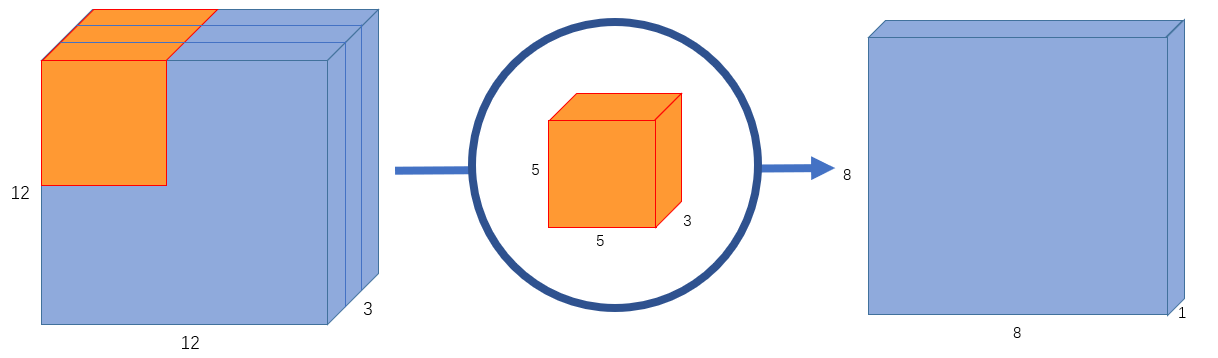
\includegraphics[width=1\textwidth]{figures/normalconvolution2.png}
    \caption{Normal convolution}
    \label{fig:normconv}
\end{figure}

Therefore if we want to have a feature map with more dimensions then we need to apply more kernels. If we want a feature map with 256 channels then we have to apply the 5x5x3 kernel 256 times. Normally this is how convolution works but this is not the case with the MobileNets architecture. MobileNets is using this approach just once at the very first layer. In all other layers it employees the depthwise separable convolution with two parts: depthwise convolution and pointwise convolution. 



\subsubsection{Depthwise convolution}
 

With depthwise convolution instead of applying one kernel with 3 channels we apply 3 kernels with one channel. Here we do not combine the three channels but perform it separately. This makes it easier to create a feature map with multiple channels. With normal convolution to achieve this we have to apply the kernel with 3 channels 3 times, but here the number of kernels stays the same but with linear time complexity. 
The advantage is to filter each input channel separately for edge detecting and so on. 



\begin{figure}[!htb]
    \centering
    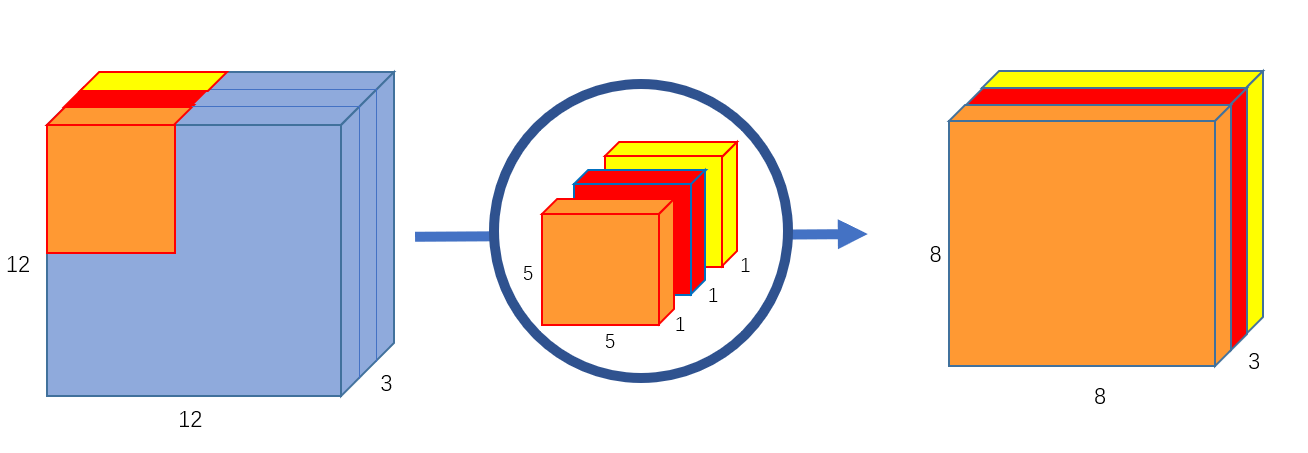
\includegraphics[width=1\textwidth]{figures/depthwise2.png}
    \caption{Depthwise convolution}
    \label{fig:depthconv}
\end{figure}

\subsubsection{Pointwise convolution}
As of now we have transformed the image into 8x8x3
So now if we want to increase the number of channels to 256 as in normal convolution above we apply a pointwise convolution. As the name say pointwise convolution applies a kernel of size 1x1x3. At this step we come back again to normal convolution, so now we apply the kernel to the image 8x8x3 from Figure~\ref{fig:depthconv} and combine it to form a one channel image with output a 8x8x1. To get 256 channels we apply the same kernel 256 times. Now we have the same feature map as in normal convolution above but with less number of computations. 

Here is a simple calculation of the both approaches, normal convolution and MobileNet approach. 
Assuming we have an input image of size 12x12x3 and the kernel is of size 5x5 and stride 1, with these parameters we will get an image of size 8x8.
With normal convolution since the input image has 3 channels we apply the kernel 5x5x3 we get an output image of size 8x8x1. If we want an image with 126 channels, the total multiplications will be as follows 126x3x5x5x8x8=604800. With the MobileNets we have 126x1x1x3x8x8=24192. Hence with MobileNets the network performs faster.


\section{Face Recognition Model Based on Convolutional Neural Network}

Face recognition is done using MobileFaceNet which consists of MobileNetv2 and ArcFace algorithm. The output of face detection is the aligned face with human face coordinates: bounding box with image and landmarks. This output will be the input for face recognition. Only if human is detected with the above mentioned model then face recognition algorithm will fire which will generate a Face ID. In order to verify who that person is, it first has to check if that person exist in the database. The next step is to compare the newly generated Face ID with the existing Face IDs. Most likely there will not be an exact match for Face IDs even if it is from the same person. So the idea is to obtain the distance between the Face IDs which is done by Euclidean distance. In order to determine if the Face ID is from the same person it will compare the distance between the Face IDs based on allowed threshold. 

\subsection{MobileFaceNet for face recognition using CNN}
MobileFaceNet is one of state of the art approaches for face verification developed by the same authors who developed MobileNet. Regarding this approach they also published a paper. MobileFaceNet is claimed to be one of the very efficient CNN model which addresses high-accuracy real-time face verification on embedded devices. Offline face verification is important on mobile devices because many applications equipped with face recognition need to run offline. 
MobileFaceNets uses around one million parameters and can achieve a very high accuracy with 99.55 percent for face verification after being trained with ArcFace algorithm. The MobileFaceNet model takes the advantage of a global
depthwise convolution layer rather than a global average pooling layer or a fully
connected layer to output a discriminative feature 512-d vector. 

Typically during face verification the models preprocess the images by extracting face features and eventually compare the new generated Face ID or vector with the already saved Face IDs by either comparing the similarities or the distance. Similarly MobileNetV2 is used here also for face feature embedding. The face verification process as seen in Figure~\ref{fig:face_ver} starts the with MTCNN and then after a face is detected with its landmarks then the aligned face is created. The aligned face is the bounding box with the face detected in size 112x112 which is then then used as an input for face reocognition. The aligned face is then mapped to a feature vector. 


\begin{figure}[!htb]
    \centering
    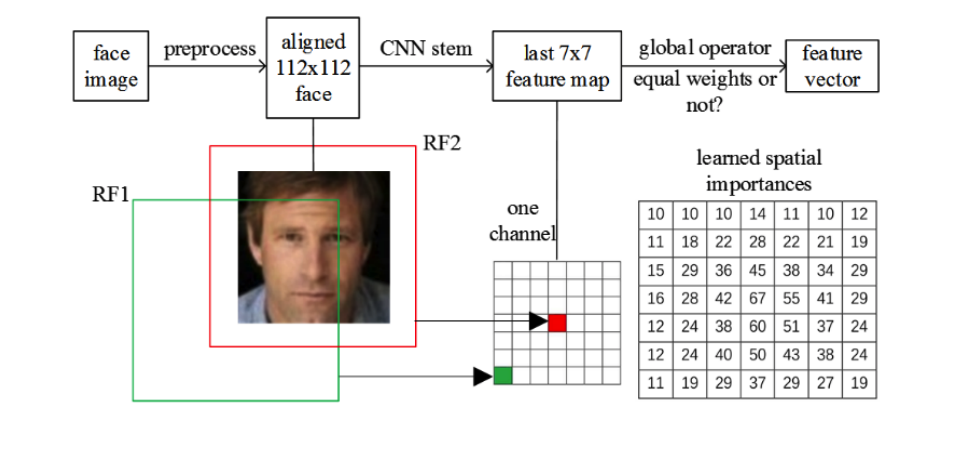
\includegraphics[width=1\textwidth]{figures/face_recognition.png}
    \caption{Face verification}
    \label{fig:face_ver}
\end{figure}

The MobileNetv2 is used similarly as in face detection up to the last feature map with size 7x7. At this step a Global Depthwise Convolution takes places, which uses a kernel of the same size as the input size. The output of this convolution is a 1x1xC while C being the number of channels. The reason behind using this approach in the last convolutional layer is that it reduces the last feature map to a vector. Which is then used as an identity for a person and the model uses it for facial recognition by computing the euclidean distance of this vector and other vectors. 